\PassOptionsToPackage{unicode=true}{hyperref} % options for packages loaded elsewhere
\PassOptionsToPackage{hyphens}{url}
\PassOptionsToPackage{dvipsnames,svgnames*,x11names*}{xcolor}
%
\documentclass[paper=a4,justified,a4paper]{tufte-handout}
\usepackage{lmodern}
\usepackage{amssymb,amsmath}
\usepackage{ifxetex,ifluatex}
\usepackage{fixltx2e} % provides \textsubscript
\ifnum 0\ifxetex 1\fi\ifluatex 1\fi=0 % if pdftex
  \usepackage[T1]{fontenc}
  \usepackage[utf8]{inputenc}
  \usepackage{textcomp} % provides euro and other symbols
\else % if luatex or xelatex
  \usepackage{unicode-math}
  \defaultfontfeatures{Ligatures=TeX,Scale=MatchLowercase}
\fi
% use upquote if available, for straight quotes in verbatim environments
\IfFileExists{upquote.sty}{\usepackage{upquote}}{}
% use microtype if available
\IfFileExists{microtype.sty}{%
\usepackage[]{microtype}
\UseMicrotypeSet[protrusion]{basicmath} % disable protrusion for tt fonts
}{}
\IfFileExists{parskip.sty}{%
\usepackage{parskip}
}{% else
\setlength{\parindent}{0pt}
\setlength{\parskip}{6pt plus 2pt minus 1pt}
}
\usepackage{xcolor}
\usepackage{hyperref}
\hypersetup{
            pdftitle={Assignment 8 Evaluate your coaching skills - Reflection Report},
            pdfauthor={Helena Rasche},
            colorlinks=true,
            linkcolor=Maroon,
            filecolor=Maroon,
            citecolor=Blue,
            urlcolor=Blue,
            breaklinks=true}
\urlstyle{same}  % don't use monospace font for urls
\usepackage{longtable,booktabs}
% Fix footnotes in tables (requires footnote package)
\IfFileExists{footnote.sty}{\usepackage{footnote}\makesavenoteenv{longtable}}{}
\usepackage{graphicx,grffile}
\makeatletter
\def\maxwidth{\ifdim\Gin@nat@width>\linewidth\linewidth\else\Gin@nat@width\fi}
\def\maxheight{\ifdim\Gin@nat@height>\textheight\textheight\else\Gin@nat@height\fi}
\makeatother
% Scale images if necessary, so that they will not overflow the page
% margins by default, and it is still possible to overwrite the defaults
% using explicit options in \includegraphics[width, height, ...]{}
\setkeys{Gin}{width=\maxwidth,height=\maxheight,keepaspectratio}
\setlength{\emergencystretch}{3em}  % prevent overfull lines
\providecommand{\tightlist}{%
  \setlength{\itemsep}{0pt}\setlength{\parskip}{0pt}}
\setcounter{secnumdepth}{0}
% Redefines (sub)paragraphs to behave more like sections
\ifx\paragraph\undefined\else
\let\oldparagraph\paragraph
\renewcommand{\paragraph}[1]{\oldparagraph{#1}\mbox{}}
\fi
\ifx\subparagraph\undefined\else
\let\oldsubparagraph\subparagraph
\renewcommand{\subparagraph}[1]{\oldsubparagraph{#1}\mbox{}}
\fi

% set default figure placement to htbp
\makeatletter
\def\fps@figure{htbp}
\makeatother

\usepackage{pdfpages}

%%%%%%%%%%% Header and Footer %%%%%%%%%%%%%%%%%%
\fancyfoot[CE,CO]{\flushright 
\includegraphics[width=3cm]{../avans.jpg}}
\fancyhead[CE,CO]{\flushleft \smallcaps{\today}}

\usepackage[]{natbib}
\bibliographystyle{plainnat}

\title{Assignment 8 Evaluate your coaching skills - Reflection Report}
\author{Helena Rasche}
\date{2022-02-07}

\begin{document}
\maketitle
\begin{abstract}
As the pandemic continues and lessons continue online, my primary
concern is that students are getting the support they need and feeling
supported. Following the experiences during BDB and with finally
beginning the period(s) during which I teach students, I've discovered a
number of points which I should remind myself of regularly as
preparation for each lesson.
\end{abstract}
\noindent\rule{5in}{0.4pt}


\hypertarget{points-of-attention}{%
\section{Points of Attention}\label{points-of-attention}}

Given that my lessons continue to be online, I find myself quite
concerned about whether or not students are getting enough support and
personal attention, and receiving it in ways that work optimally for
them. I know that students can feel significantly isolated with working
from home constantly, and that I want to ensure that I'm a friendly and
accepting person that they feel comfortable contacting when they have
issues.

\hypertarget{questionnaire}{%
\section{Questionnaire}\label{questionnaire}}

I designed the enquête to measure a couple aspects of this
communication:

\begin{itemize}
\tightlist
\item
  Preferred method(s)
\item
  Preferred interaction modalities
\item
  Their experiences as students in my class
\item
  And their feelings on my interactions with them until now.
\end{itemize}

These aspects I found to be particularly important to me and my
interactions with students. I elaborated these with the following survey
design:

\begin{longtable}[]{@{}lll@{}}
\toprule
\begin{minipage}[b]{0.30\columnwidth}\raggedright
Question\strut
\end{minipage} & \begin{minipage}[b]{0.30\columnwidth}\raggedright
Aspect\strut
\end{minipage} & \begin{minipage}[b]{0.30\columnwidth}\raggedright
Text\strut
\end{minipage}\tabularnewline
\midrule
\endhead
\begin{minipage}[t]{0.30\columnwidth}\raggedright
1\strut
\end{minipage} & \begin{minipage}[t]{0.30\columnwidth}\raggedright
Question\strut
\end{minipage} & \begin{minipage}[t]{0.30\columnwidth}\raggedright
How comfortable do you feel discussing course questions, issues,
programming questions via\strut
\end{minipage}\tabularnewline
\begin{minipage}[t]{0.30\columnwidth}\raggedright
1\strut
\end{minipage} & \begin{minipage}[t]{0.30\columnwidth}\raggedright
Description\strut
\end{minipage} & \begin{minipage}[t]{0.30\columnwidth}\raggedright
Example questions include: where's the course recording, why is my code
failing, what do you mean I need to import that first\strut
\end{minipage}\tabularnewline
\begin{minipage}[t]{0.30\columnwidth}\raggedright
1\strut
\end{minipage} & \begin{minipage}[t]{0.30\columnwidth}\raggedright
Answer\strut
\end{minipage} & \begin{minipage}[t]{0.30\columnwidth}\raggedright
A choice matrix of {[}Email, Teams Text Chat, Teams Video Chat, In
person{]} and {[}Please no!, If I must, Meh, It's ok, Yes please, My
preferred way!{]}\strut
\end{minipage}\tabularnewline
\begin{minipage}[t]{0.30\columnwidth}\raggedright
2\strut
\end{minipage} & \begin{minipage}[t]{0.30\columnwidth}\raggedright
Question\strut
\end{minipage} & \begin{minipage}[t]{0.30\columnwidth}\raggedright
I find online classes \ldots{}.\strut
\end{minipage}\tabularnewline
\begin{minipage}[t]{0.30\columnwidth}\raggedright
2\strut
\end{minipage} & \begin{minipage}[t]{0.30\columnwidth}\raggedright
Description\strut
\end{minipage} & \begin{minipage}[t]{0.30\columnwidth}\raggedright
1 = They work great for me! 5 = It's so exhausted I hate it here\strut
\end{minipage}\tabularnewline
\begin{minipage}[t]{0.30\columnwidth}\raggedright
2\strut
\end{minipage} & \begin{minipage}[t]{0.30\columnwidth}\raggedright
Answer\strut
\end{minipage} & \begin{minipage}[t]{0.30\columnwidth}\raggedright
Likert-type scale (1-5)\strut
\end{minipage}\tabularnewline
\begin{minipage}[t]{0.30\columnwidth}\raggedright
3\strut
\end{minipage} & \begin{minipage}[t]{0.30\columnwidth}\raggedright
Question\strut
\end{minipage} & \begin{minipage}[t]{0.30\columnwidth}\raggedright
How do you feel about\strut
\end{minipage}\tabularnewline
\begin{minipage}[t]{0.30\columnwidth}\raggedright
3\strut
\end{minipage} & \begin{minipage}[t]{0.30\columnwidth}\raggedright
Answer\strut
\end{minipage} & \begin{minipage}[t]{0.30\columnwidth}\raggedright
Choice matrix of {[}Breakout rooms, being randomly called on, being
predictably called on, Kahoots / Competitive quizzes{]} and feeling
matrix of {[}Hate it, Meh, It's fun{]}\strut
\end{minipage}\tabularnewline
\begin{minipage}[t]{0.30\columnwidth}\raggedright
4\strut
\end{minipage} & \begin{minipage}[t]{0.30\columnwidth}\raggedright
Question\strut
\end{minipage} & \begin{minipage}[t]{0.30\columnwidth}\raggedright
Helena wants to discuss my solution in front of the class, that makes me
feel\strut
\end{minipage}\tabularnewline
\begin{minipage}[t]{0.30\columnwidth}\raggedright
4\strut
\end{minipage} & \begin{minipage}[t]{0.30\columnwidth}\raggedright
Answer\strut
\end{minipage} & \begin{minipage}[t]{0.30\columnwidth}\raggedright
Free text\strut
\end{minipage}\tabularnewline
\begin{minipage}[t]{0.30\columnwidth}\raggedright
5\strut
\end{minipage} & \begin{minipage}[t]{0.30\columnwidth}\raggedright
Question\strut
\end{minipage} & \begin{minipage}[t]{0.30\columnwidth}\raggedright
Some of you have commented I go too quickly, how can we address
this?\strut
\end{minipage}\tabularnewline
\begin{minipage}[t]{0.30\columnwidth}\raggedright
5\strut
\end{minipage} & \begin{minipage}[t]{0.30\columnwidth}\raggedright
Description\strut
\end{minipage} & \begin{minipage}[t]{0.30\columnwidth}\raggedright
I'm guessing you don't want to publicly speak up? Would you want to
message the TOA who can ask me to slow down? Is there something I can do
to make you feel ok asking me to slow down in front of your peers? (I
need the reminder, I get too focused on covering content, for
sure.)\strut
\end{minipage}\tabularnewline
\begin{minipage}[t]{0.30\columnwidth}\raggedright
5\strut
\end{minipage} & \begin{minipage}[t]{0.30\columnwidth}\raggedright
Answer\strut
\end{minipage} & \begin{minipage}[t]{0.30\columnwidth}\raggedright
Free text\strut
\end{minipage}\tabularnewline
\begin{minipage}[t]{0.30\columnwidth}\raggedright
6\strut
\end{minipage} & \begin{minipage}[t]{0.30\columnwidth}\raggedright
Question\strut
\end{minipage} & \begin{minipage}[t]{0.30\columnwidth}\raggedright
I feel like part of the class when ?\strut
\end{minipage}\tabularnewline
\begin{minipage}[t]{0.30\columnwidth}\raggedright
6\strut
\end{minipage} & \begin{minipage}[t]{0.30\columnwidth}\raggedright
Description\strut
\end{minipage} & \begin{minipage}[t]{0.30\columnwidth}\raggedright
i.e.~specific types of activities (and that I'm getting something more
useful out of being here rather than doing chores or something
else.)\strut
\end{minipage}\tabularnewline
\begin{minipage}[t]{0.30\columnwidth}\raggedright
6\strut
\end{minipage} & \begin{minipage}[t]{0.30\columnwidth}\raggedright
Answer\strut
\end{minipage} & \begin{minipage}[t]{0.30\columnwidth}\raggedright
Free text\strut
\end{minipage}\tabularnewline
\begin{minipage}[t]{0.30\columnwidth}\raggedright
7\strut
\end{minipage} & \begin{minipage}[t]{0.30\columnwidth}\raggedright
Question\strut
\end{minipage} & \begin{minipage}[t]{0.30\columnwidth}\raggedright
Any other remarks?\strut
\end{minipage}\tabularnewline
\begin{minipage}[t]{0.30\columnwidth}\raggedright
7\strut
\end{minipage} & \begin{minipage}[t]{0.30\columnwidth}\raggedright
Answer\strut
\end{minipage} & \begin{minipage}[t]{0.30\columnwidth}\raggedright
Free text\strut
\end{minipage}\tabularnewline
\begin{minipage}[t]{0.30\columnwidth}\raggedright
8\strut
\end{minipage} & \begin{minipage}[t]{0.30\columnwidth}\raggedright
Question\strut
\end{minipage} & \begin{minipage}[t]{0.30\columnwidth}\raggedright
Are you getting the support you need? Do you have the resources you
need?\strut
\end{minipage}\tabularnewline
\begin{minipage}[t]{0.30\columnwidth}\raggedright
8\strut
\end{minipage} & \begin{minipage}[t]{0.30\columnwidth}\raggedright
Answer\strut
\end{minipage} & \begin{minipage}[t]{0.30\columnwidth}\raggedright
Likert-type scale with stars (1-5)\strut
\end{minipage}\tabularnewline
\begin{minipage}[t]{0.30\columnwidth}\raggedright
9\strut
\end{minipage} & \begin{minipage}[t]{0.30\columnwidth}\raggedright
Question\strut
\end{minipage} & \begin{minipage}[t]{0.30\columnwidth}\raggedright
Final Remarks?\strut
\end{minipage}\tabularnewline
\begin{minipage}[t]{0.30\columnwidth}\raggedright
9\strut
\end{minipage} & \begin{minipage}[t]{0.30\columnwidth}\raggedright
Answer\strut
\end{minipage} & \begin{minipage}[t]{0.30\columnwidth}\raggedright
Free text\strut
\end{minipage}\tabularnewline
\bottomrule
\end{longtable}

\hypertarget{results}{%
\subsection{Results}\label{results}}

\begin{figure}
\centering
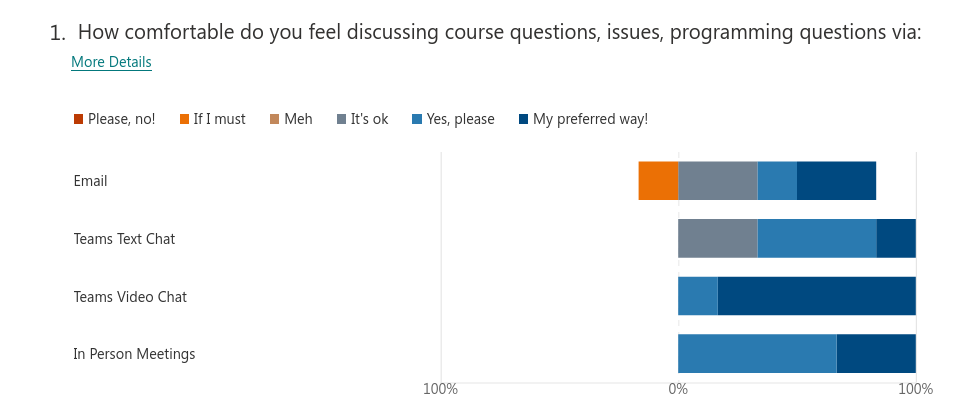
\includegraphics{./q1.png}
\caption{Students seem to be extremely}
\end{figure}

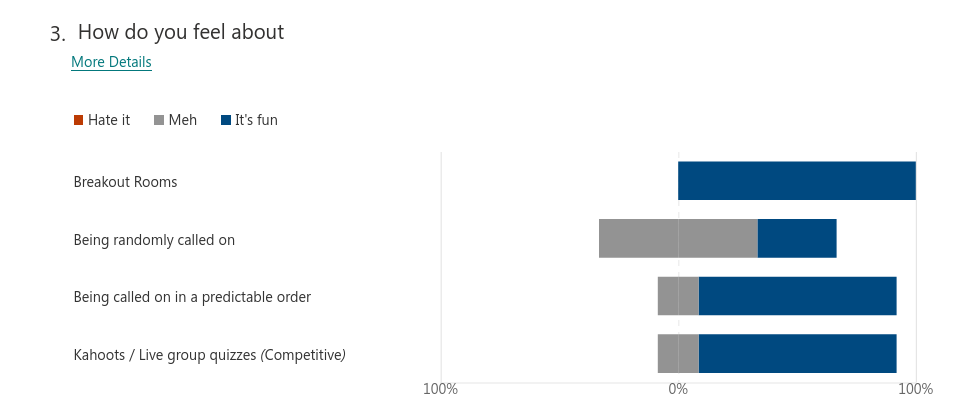
\includegraphics{./q3.png}

\begin{enumerate}
\def\labelenumi{\arabic{enumi}.}
\setcounter{enumi}{3}
\tightlist
\item
  Process and describe the results and reflect on them via a reflection
  model of your choice.
\item
  Formulate action points: to what and how do you want to work in
  relation to the teacher-student relationship?
\item
  Submit a report of the above (1, 4 and 5) and the questionnaire (2) in
  your portfolio.
\end{enumerate}

\bibliography{report.bib}

\end{document}
